\documentclass{beamer}
%Information to be included in the title page:
\usetheme{default}
% \setbeamertemplate{background canvas}{\includegraphics
% 	[width=\paperwidth]{uclheader.pdf}}
	
% \definecolor{bluecolour}{rgb}{0.19,0.52,0.98}
% \useinnertheme[shadow=true]{rounded}
% \setbeamertemplate{items}[circle]
% \setbeamercolor{title}{bg=bluecolour, fg=black}
% \setbeamercolor{structure}{fg=bluecolour}
\usepackage{helvet}
\title{Weekly meeting}
\subtitle{Meeting 2}
\date{31st October 2023}


\begin{document}

\frame{\titlepage}

\begin{frame}{Frame Title}
\frametitle{Table of Contents}
\tableofcontents
\end{frame}


\section{Progress this week}
\begin{frame}
\frametitle{Progress this week}
\begin{figure}
    \centering
    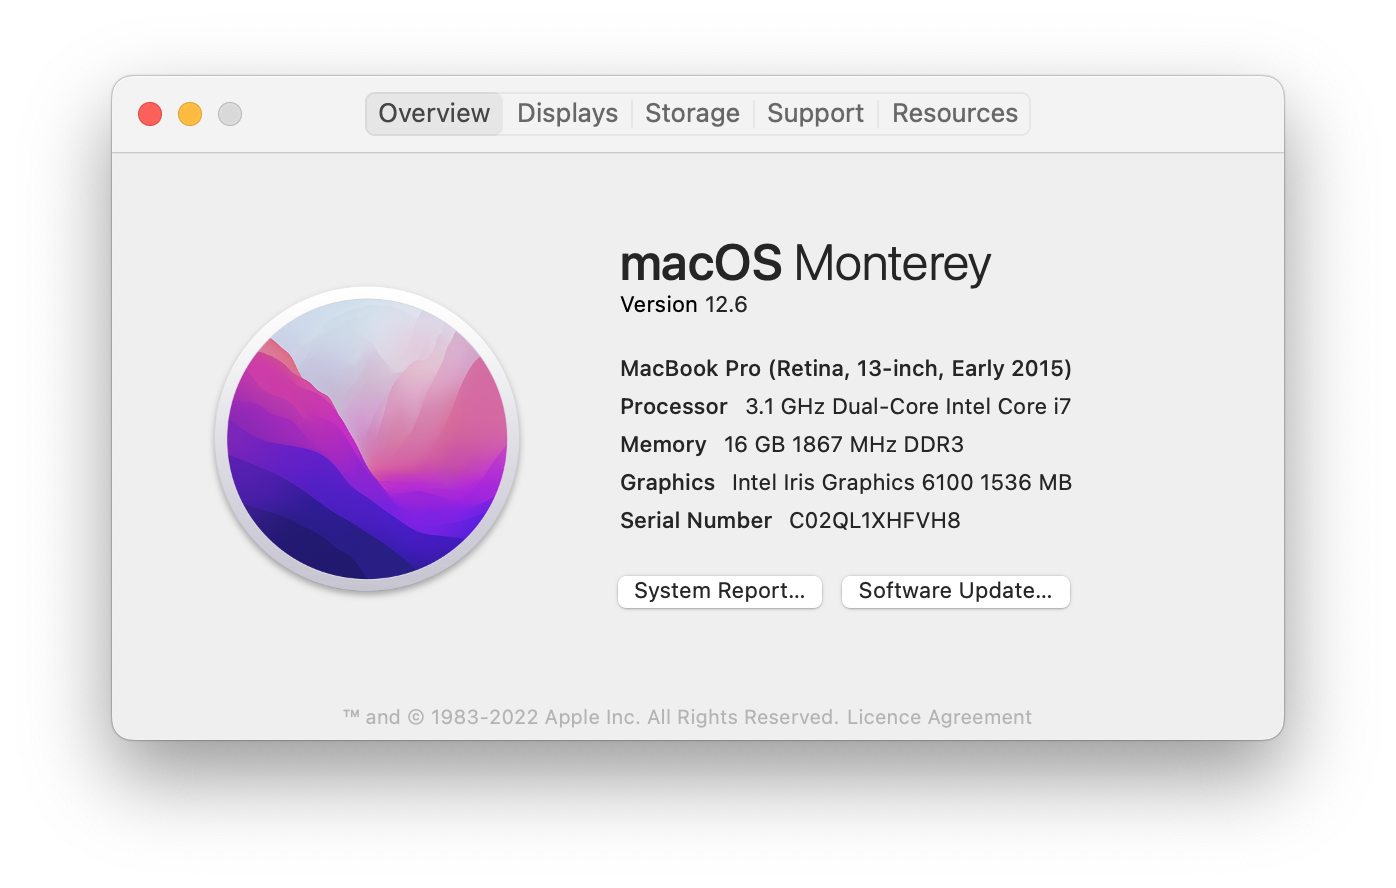
\includegraphics[scale=0.15]{Weekly meeting slides/Screenshot 2023-10-27 at 10.20.22 am.png}
    \label{fig:enter-label}
\end{figure}
Expected to spend 10-15 hours a week

attempted things one

attempted things two
\end{frame}

\begin{frame}{Problems this week}
    
\end{frame}

\section{Plan for next week}
\begin{frame}{Plan for next week}
    Project outline due on 3rd of November
\end{frame}

\section{Questions}

\begin{frame}{Questions}
    
\end{frame}

\end{document}